% !TEX TS-program = xelatex
\documentclass[aspectratio=169,10pt]{beamer}

\usepackage{fontspec}
\usepackage{polyglossia}
\setmainlanguage{russian}
\setotherlanguage{english}
\setsansfont{DejaVu Sans}
\setmonofont{DejaVu Sans Mono}

\usepackage{amsmath}
\usepackage{booktabs}
\usepackage{graphicx}
\usepackage{hyperref}
\usepackage{xcolor}

\graphicspath{{results/figures/}{results/raw_video_demo/}}

\usetheme{Madrid}
\usecolortheme{seahorse}
\setbeamertemplate{navigation symbols}{}
\setbeamertemplate{footline}[frame number]

\definecolor{mainblue}{HTML}{2563EB}
\definecolor{mainred}{HTML}{DC2626}
\definecolor{muted}{HTML}{64748B}
\setbeamercolor{title}{fg=mainblue}
\setbeamercolor{frametitle}{fg=mainblue}
\setbeamercolor{structure}{fg=mainblue}

\title[Прогнозирование действий по RGB-признакам]{Краткосрочное прогнозирование событий в эгоцентрическом видео по извлечённым RGB-признакам}
\subtitle{EPIC-KITCHENS-55 / RULSTM features, next-action anticipation}
\author{\textbf{Сулиман Адам}}
\date{\today}

\newcommand{\metric}[1]{\textbf{#1}}
\newcommand{\todo}[1]{\textcolor{mainred}{TODO: #1}}

\begin{document}

\begin{frame}
    \titlepage
\end{frame}

\begin{frame}{Задача}
    \begin{block}{Формулировка}
        По короткой наблюдаемой последовательности визуальных признаков нужно предсказать следующее действие пользователя в эгоцентрическом видео.
    \end{block}

    \[
        X = (f_1, \ldots, f_T), \quad f_t \in \mathbb{R}^{1024}
    \]

    \[
        y = (v, n), \quad v = \text{verb}, \quad n = \text{noun}
    \]

    \begin{itemize}
        \item Вход: последовательность RGB-признаков до следующего действия.
        \item Выход: глагол, существительное и совместная пара \((v,n)\).
        \item Цель: получить эффективную модель для ограниченных вычислительных ресурсов.
    \end{itemize}
\end{frame}

\begin{frame}{Мотивация и ограничения}
    \begin{itemize}
        \item Полное обучение на raw video требует дорогого backbone и большого количества времени и ресурсов.
        \item Доступная среда: Kaggle kernel, до 2x T4, около 30 GiB RAM, ограниченное время.
        \item Основной эксперимент: \textbf{feature-based anticipation}, не требует обучения визуального backbone, всё ещё давая хорошие результаты в egocentric action anticipation.
        \item Мы не обучаем визуальный backbone.
    \end{itemize}

    \vspace{0.4cm}
    \begin{block}{Исследовательский вопрос}
        Можно ли улучшить краткосрочное прогнозирование следующего действия, используя компактную temporal модель поверх фиксированных RGB-признаков?
    \end{block}
\end{frame}

\begin{frame}{Данные}
    \begin{itemize}
        \item Использован набор: \textbf{EPIC-KITCHENS-55 RULSTM RGB pre-extracted features}.
        \item Это не raw video, а предвычисленные признаки из RGB-потока.
        \item Каждый sample имеет форму:
        \[
            14 \times 1024
        \]
        \item 14 временных фрагментов перед действием, 1024 признака на фрагмент.
    \end{itemize}

    \vspace{0.25cm}
    \begin{table}
        \centering
        \begin{tabular}{lr}
            \toprule
            Параметр & Кол-во \\
            \midrule
            Train samples & 23,472 \\
            Validation samples & 4,972 \\
            Verb classes & 119 \\
            Noun classes & 321 \\
            Seen train actions & 2,288 \\
            \bottomrule
        \end{tabular}
    \end{table}
\end{frame}

\begin{frame}{Что такое RGB-признаки}
    \begin{itemize}
        \item RGB-признаки --- это численные векторы, заранее извлеченные из обычных цветных кадров.
        \item В RULSTM эти признаки извлечены с помощью \textbf{BN-Inception CNN}, обученной для egocentric action recognition в схеме \textbf{Temporal Segment Networks (TSN)}.
        \item Используется только RGB stream; flow/object признаки в основных экспериментах не используются.
        \item Схема получения признаков:
        \[
            \text{RGB frames} \rightarrow \text{TSN BN-Inception} \rightarrow f_t \in \mathbb{R}^{1024}
        \]
        \item Наша работа начинается после этого этапа:
        \[
            (f_1,\ldots,f_{14}) \rightarrow \text{temporal model} \rightarrow (v,n)
        \]
        \item Поэтому вклад проекта --- не feature extraction, а эффективное temporal/action-level modeling поверх фиксированных RGB features.
    \end{itemize}
\end{frame}

\begin{frame}{Метрики качества}
    \small
    \begin{block}{Top-k accuracy}
        Для каждого validation sample модель ранжирует возможные ответы по score.
        Top-k засчитывается как 1, если правильный ответ входит в первые \(k\) кандидатов.
    \end{block}

    \begin{itemize}
        \item \metric{Verb top-1 / top-5}: правильно ли предсказан глагол, например \textit{open}, \textit{take}, \textit{put}.
        \item \metric{Noun top-1 / top-5}: правильно ли предсказан объект действия, например \textit{drawer}, \textit{knife}, \textit{plate}.
        \item \metric{Joint action top-1 / top-5}: правильно ли предсказана вся пара \((v,n)\).
        Это главная метрика: для next-action anticipation важно угадать не только действие, но и объект.
    \end{itemize}

    \vspace{0.15cm}
    Joint action top-k считается по матрице всех verb-noun пар:
    \[
        S_{v,n} = s_v + s_n + \lambda \log P_{\text{train}}(v,n) + \gamma s_{a(v,n)}
    \]
    \footnotesize
    Здесь \(s_v, s_n\) --- logits отдельных голов, \(\log P_{\text{train}}\) --- статистический prior,
    \(s_a\) --- score action-head для seen action pairs.
\end{frame}

\begin{frame}{Метрики эффективности}
    \small
    \begin{itemize}
        \item \metric{Число обучаемых параметров}: размер temporal model без frozen RGB backbone.
        Показывает, насколько модель компактна.
        \item \metric{Время обучения на эпоху}: wall-clock время одного прохода по train split.
        \item \metric{Inference time per validation sample}: среднее время предсказания на один validation sample.
        Это важно для сценария online anticipation.
        \item \metric{Peak GPU memory}: максимальная выделенная CUDA-память во время запуска.
    \end{itemize}

    \vspace{0.25cm}
    \begin{block}{Почему качество и эффективность показываются вместе}
        Цель проекта --- не максимизация accuracy любой ценой, а хороший компромисс:
        улучшить joint action top-5 при малом числе параметров, быстром обучении и небольшом расходе GPU memory.
    \end{block}
\end{frame}

\begin{frame}{Сравниваемые методы}
    \small
    \begin{enumerate}
        \item \textbf{Prior-only}: не использует \(X\), а ранжирует пары по сглаженной частоте
        \(P_{\text{train}}(v,n)\). Это нижняя граница ``только статистика labels''.
        \item \textbf{MeanPool MLP}: заменяет последовательность средним вектором
        \(\bar f = \frac{1}{T}\sum_t f_t\). Проверяет, достаточно ли общего визуального контекста без порядка кадров.
        \item \textbf{GRU}: читает признаки по времени и хранит скрытое состояние \(h_t\).
        Проверяет вклад temporal order и динамики перед действием.
        \item \textbf{TinyRMT / AttentiveGRU}: добавляют память или attention поверх короткой последовательности.
        Проверяют, помогает ли выбор важных временных фрагментов.
        \item \textbf{JointGRU}: GRU + auxiliary head для seen verb-noun pairs.
        Добавляет прямой score для joint action, а не только сумму verb и noun logits.
    \end{enumerate}

    \vspace{0.25cm}
    \begin{block}{Логика сравнения}
        Идем от статистического baseline к временной модели и затем к модели,
        которая явно учитывает совместимость verb-noun пары.
    \end{block}
\end{frame}

\begin{frame}{Предложенный метод: JointGRU}
    \small
    \begin{columns}
        \begin{column}{0.52\textwidth}
            \begin{itemize}
                \item На шаге \(t\) GRU получает текущий RGB-признак \(f_t\) и прошлую память \(h_{t-1}\).
                \item \textbf{Update gate} \(z_t\) решает, сколько новой информации записать.
                \item \textbf{Reset gate} \(r_t\) решает, какую часть прошлой памяти использовать.
                \item После последнего шага \(h_T\) --- компактное описание наблюдаемого контекста перед следующим действием.
                \item Из \(h_T\) строятся три головы:
                \begin{itemize}
                    \item verb head;
                    \item noun head;
                    \item seen-action head.
                \end{itemize}
            \end{itemize}
        \end{column}
        \begin{column}{0.48\textwidth}
            \scriptsize
            \[
            \begin{aligned}
                z_t &= \sigma(W_z f_t + U_z h_{t-1}) \\
                r_t &= \sigma(W_r f_t + U_r h_{t-1}) \\
                \tilde h_t &= \tanh(W_h f_t + U_h(r_t \odot h_{t-1})) \\
                h_t &= (1-z_t)\odot h_{t-1} + z_t\odot \tilde h_t
            \end{aligned}
            \]

            \vspace{0.05cm}
            \[
                s_v = W_v h_T,\quad
                s_n = W_n h_T,\quad
                s_a = W_a h_T
            \]
            \[
                S_{v,n} =
                s_v(v) + s_n(n)
                + \lambda \log P(v,n)
                + \gamma s_a(v,n)
            \]
            \footnotesize
            Action head обучается только на парах \((v,n)\), встреченных в train;
            для unseen пар остается сумма verb/noun score и prior.
        \end{column}
    \end{columns}
\end{frame}

\begin{frame}{Функция потерь}
    \[
        \mathcal{L} =
        \mathrm{CE}(s_v, v)
        + \mathrm{CE}(s_n, n)
        + \beta \mathrm{CE}(s_a, a)
    \]

    \vspace{-0.1cm}
    \[
        \mathrm{CE}(s, y) = - \log
        \frac{\exp(s_y)}{\sum_j \exp(s_j)}
    \]

    \begin{itemize}
        \item \(s_v \in \mathbb{R}^{119}\): logits по классам глаголов, \(v\) --- истинный verb label.
        \item \(s_n \in \mathbb{R}^{321}\): logits по классам существительных, \(n\) --- истинный noun label.
        \item \(s_a \in \mathbb{R}^{2288}\): logits по verb-noun парам, встреченным в train; \(a\) --- индекс истинной пары.
        \item Cross-entropy штрафует модель, если logit истинного класса мал относительно остальных logits.
        \item \(\beta\) управляет вкладом auxiliary action head: для обычных baseline \(\beta=0\), для JointGRU \(\beta=0.3\).
    \end{itemize}
\end{frame}

\begin{frame}{Основные результаты}
    \begin{table}
        \centering
        \small
        \begin{tabular}{lrrrr}
            \toprule
            Метод & Params & ms/sample & Action@1 & Action@5 \\
            \midrule
            Prior-only & 0 & 0.164 & 0.026 & 0.082 \\
            MeanPool MLP & 1.01M & 0.103 & 0.111 & 0.286 \\
            TinyRMT-256 & 0.91M & 0.100 & 0.142 & 0.304 \\
            GRU-384 & 1.79M & 0.105 & 0.154 & 0.326 \\
            GRU-512 & 2.59M & 0.099 & 0.156 & 0.328 \\
            GRU-768 & 4.47M & 0.102 & 0.158 & 0.335 \\
            JointGRU-768 & 6.23M & 0.113 & 0.168 & \textbf{0.360} \\
            \bottomrule
        \end{tabular}
    \end{table}

    \vspace{0.2cm}
    Лучший результат: JointGRU-768, \( \lambda=0.1, \gamma=2.0 \), Action@5 \(=0.360 \pm 0.006\).
\end{frame}

\begin{frame}{Качество: Action top-5}
    \centering
    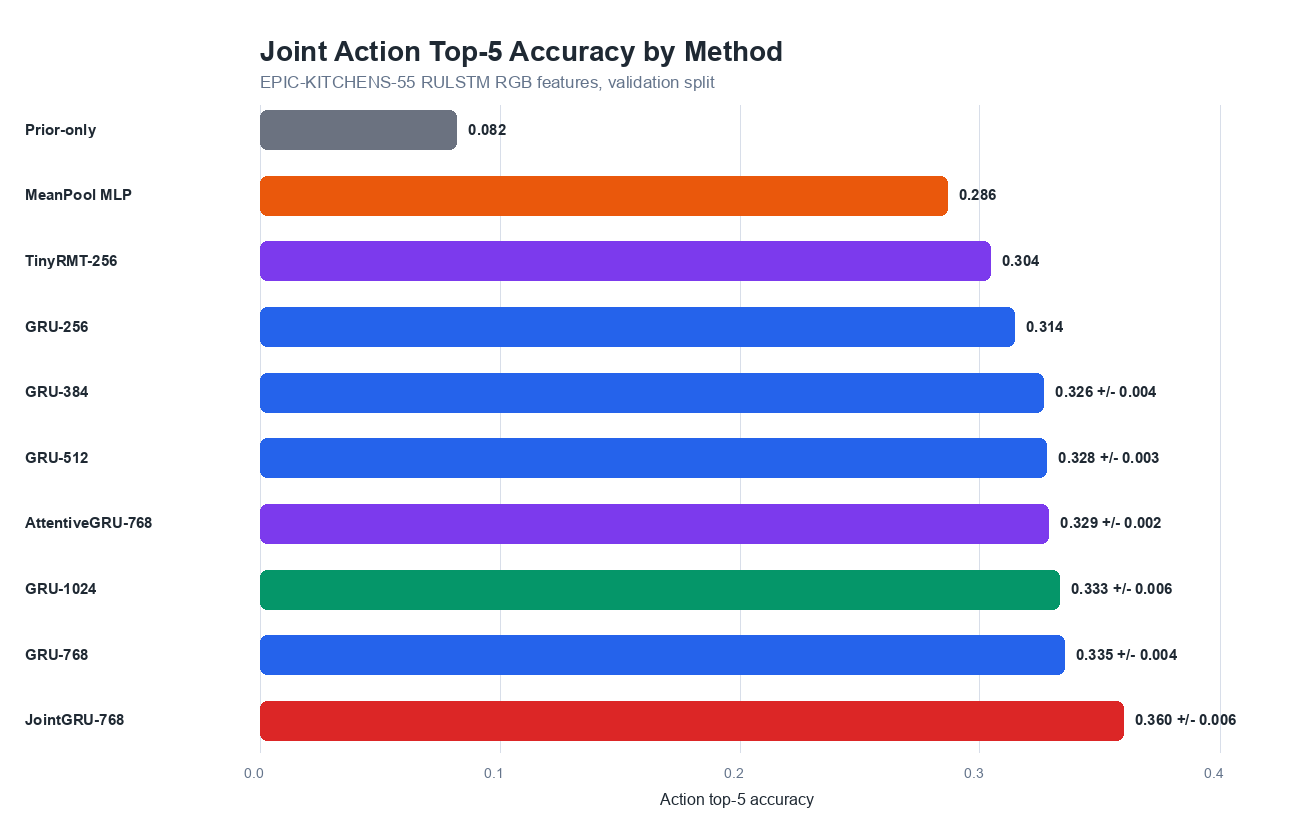
\includegraphics[height=0.78\textheight,keepaspectratio]{main_action_top5_comparison.png}
\end{frame}

\begin{frame}{Качество против эффективности}
    \centering
    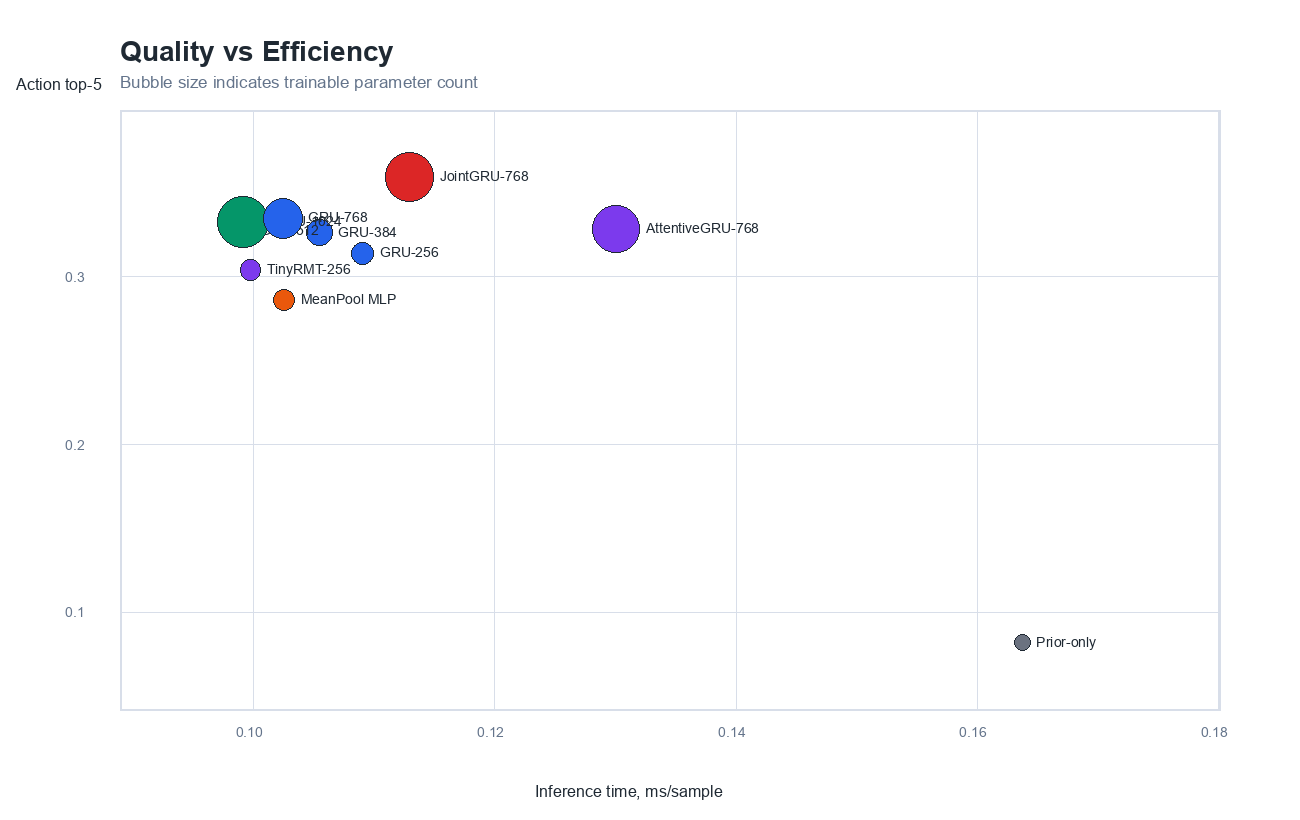
\includegraphics[height=0.78\textheight,keepaspectratio]{quality_efficiency_tradeoff.png}
\end{frame}

\begin{frame}{Ablation: статистический prior}
    \centering
    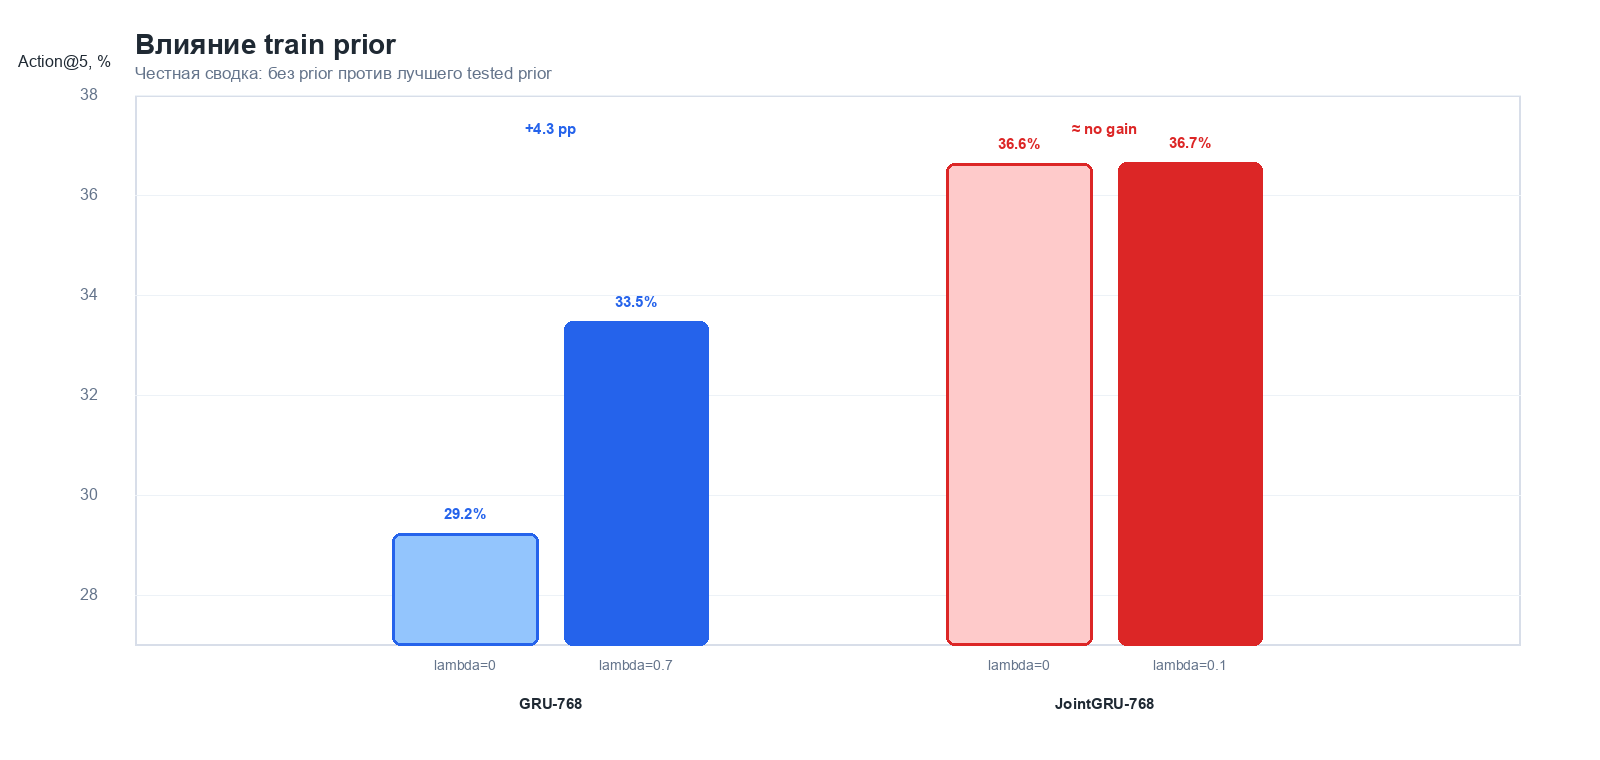
\includegraphics[width=0.9\textwidth,keepaspectratio]{prior_effect_ablation.png}

    \scriptsize
    \parbox{0.9\textwidth}{
        Чтобы не сравнивать 7 точек GRU против 3 точек JointGRU, показана сводка:
        качество без prior и лучший tested prior. Prior дает большой прирост plain GRU,
        но почти не улучшает JointGRU, где совместимость пары уже моделируется action head.
    }
\end{frame}

\begin{frame}{Ablation: action-score fusion}
    \centering
    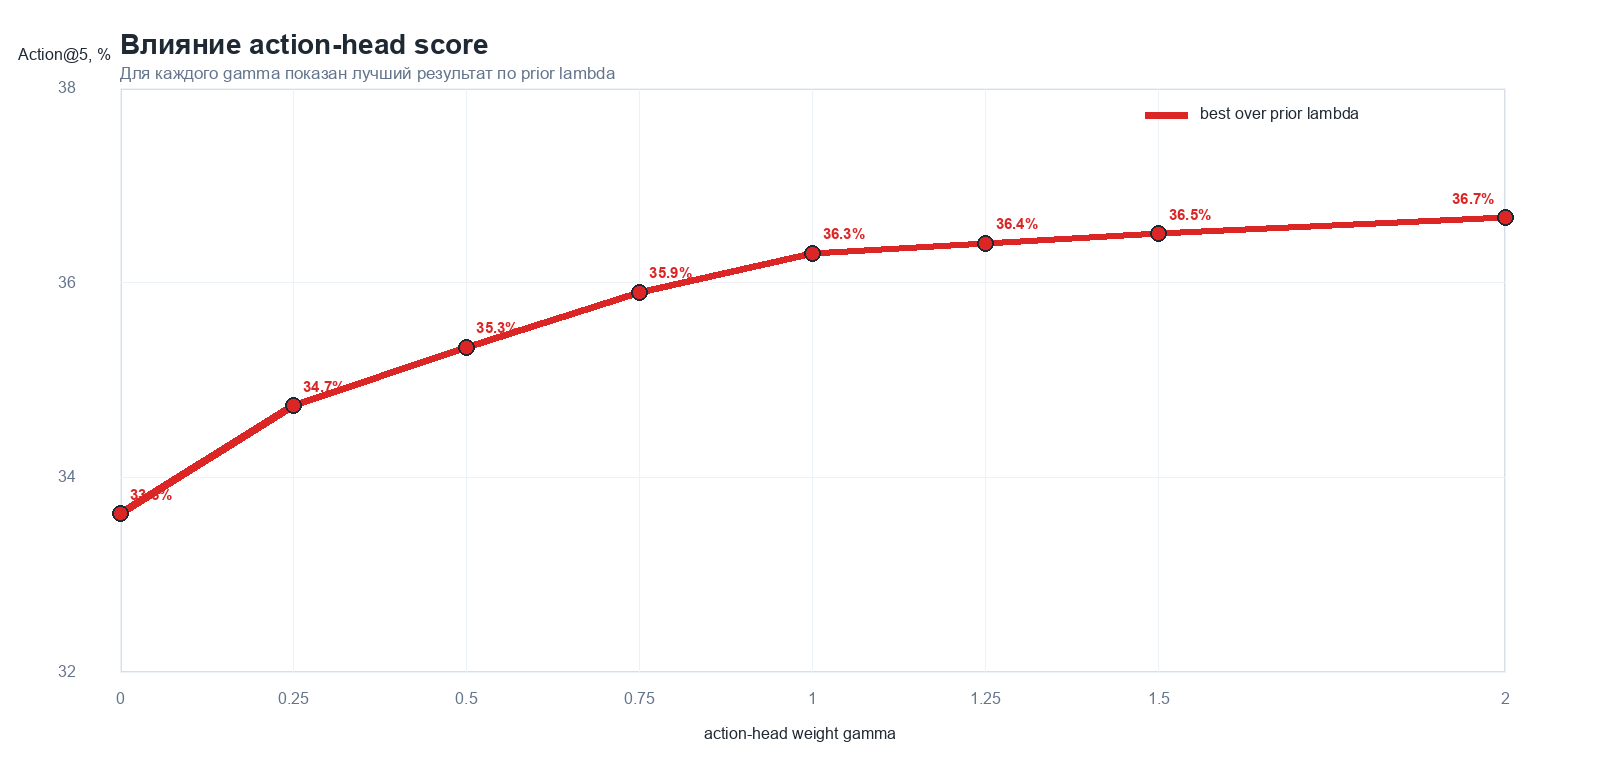
\includegraphics[width=0.9\textwidth,keepaspectratio]{action_score_weight_ablation.png}

    \scriptsize
    \parbox{0.9\textwidth}{
        Увеличение веса action head дает основной прирост до \( \gamma \approx 1.0 \);
        дальше качество растет медленнее, но лучший запуск получился при \( \gamma=2.0 \).
    }
\end{frame}

\begin{frame}{Качественный пример: validation sample 10}
    \centering
    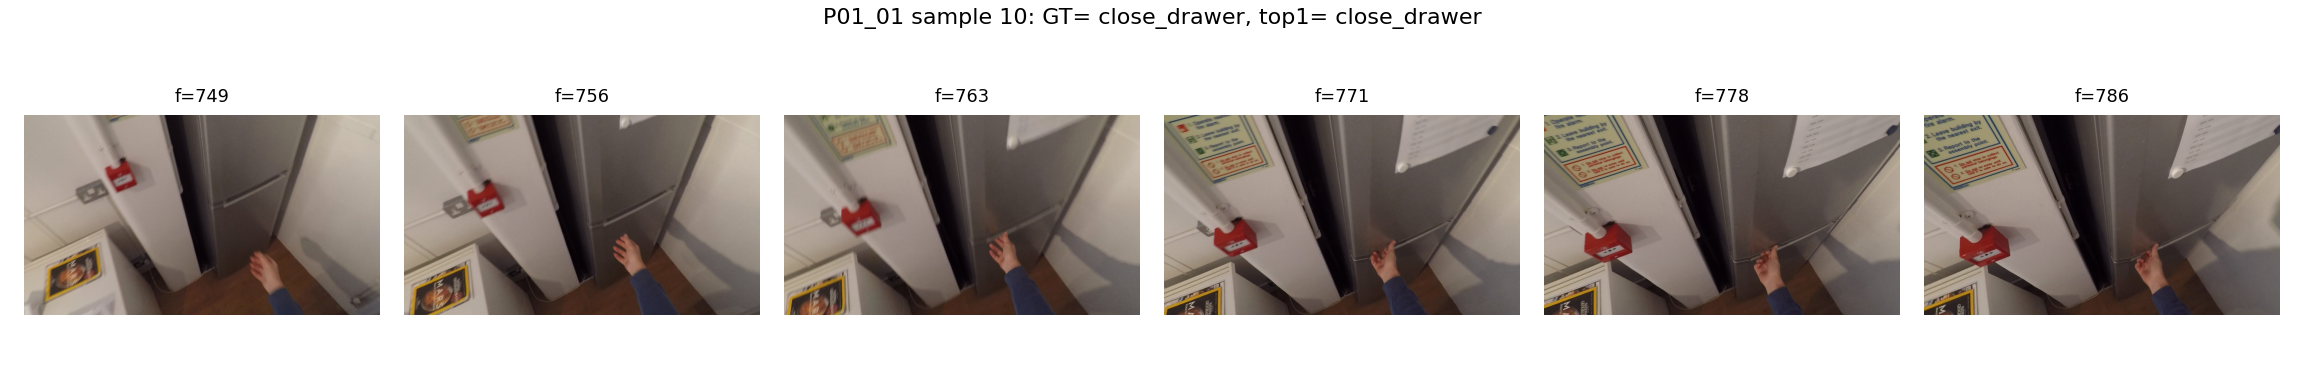
\includegraphics[width=0.96\textwidth,keepaspectratio]{sample_00010_P01_01.png}

    \vspace{0.12cm}
    \small
    \begin{tabular}{lll}
        \toprule
        Ранг & Предсказанная пара & Комментарий \\
        \midrule
        1 & \textbf{close\_drawer} & совпадает с ground truth \\
        2 & open\_drawer & близкое действие с тем же объектом \\
        3 & close\_door & похожий verb, другой noun \\
        5 & take\_drawer & тот же объект, другой verb \\
        \bottomrule
    \end{tabular}

    \vspace{0.1cm}
    \footnotesize
    Кадры используются только для визуализации; предсказание сделано по соответствующим RULSTM RGB-признакам.
\end{frame}

\begin{frame}{Интерпретация результатов}
    \begin{itemize}
        \item Статистика train labels сама по себе слаба: Prior-only Action@5 = 0.082.
        \item MeanPool уже дает разумный baseline: Action@5 = 0.286.
        \item GRU улучшает качество за счет временного порядка: Action@5 = 0.335.
        \item Простое увеличение hidden size до 1024 не помогает.
        \item Attention/TinyRMT не превзошли plain GRU.
        \item JointGRU улучшает качество за счет дополнительной action-level supervision.
    \end{itemize}

    \vspace{0.2cm}
    \begin{block}{Главный вывод}
        При фиксированных RGB-признаках важен не только temporal encoder, но и согласование factorized verb/noun prediction с совместной action pair prediction.
    \end{block}
\end{frame}

\begin{frame}{Ограничения}
    \begin{itemize}
        \item Модель не обучается на raw video frames.
        \item RGB backbone фиксирован и не дообучается.
        \item Используются только RGB-признаки: без optical flow, audio, object detections.
        \item Результаты являются validation performance, не test-server performance.
        \item Hyperparameters подбирались по validation set, поэтому validation не является полностью untouched final test.
    \end{itemize}

    \vspace{0.25cm}
    \begin{block}{Почему это все равно корректно}
        Задача и labels реальные: EPIC-KITCHENS-55 validation action anticipation. Ограничение касается только того, что визуальный backbone уже предвычислен.
    \end{block}
\end{frame}

\begin{frame}{Вклад участника}
    \begin{itemize}
        \item Подготовлен Kaggle-compatible экспериментальный pipeline.
        \item Реализованы data discovery, feature dataset loader и synthetic fallback.
        \item Реализованы baselines: Prior-only, MeanPool MLP, GRU, TinyRMT/AttentiveGRU.
        \item Разработан и проверен JointGRU с auxiliary seen-action head.
        \item Реализованы joint action top-k metrics и efficiency metrics.
        \item Проведены seed sweeps, ablations и анализ результатов.
        \item Подготовлены финальные таблицы и графики для презентации.
    \end{itemize}
\end{frame}

\begin{frame}{Репозиторий и воспроизводимость}
    \begin{itemize}
        \item Основной notebook:
        \[
            \texttt{video\_event\_prediction\_rgb\_features\_experiments.ipynb}
        \]
        \item VS Code Python notebook:
        \[
            \texttt{video\_event\_prediction\_rgb\_features\_experiments.py}
        \]
        \item Скрипт графиков:
        \[
            \texttt{results/make\_presentation\_figures.py}
        \]
        \item Результаты:
        \[
            \texttt{results/final\_results\_table.csv}
        \]
    \end{itemize}

    \vspace{0.2cm}
    \todo{вставить ссылку на GitHub/Kaggle notebook перед сдачей}
\end{frame}

\begin{frame}{Итог}
    \begin{itemize}
        \item Построен компактный pipeline для next-action anticipation по RGB-признакам.
        \item Получено сравнение аналитического baseline и нескольких нейросетевых методов.
        \item Лучший метод: JointGRU-768 с auxiliary action head.
        \item Улучшение над сильным GRU-768 baseline:
        \[
            0.335 \rightarrow 0.360 \quad \text{Action@5}
        \]
        \item Метод остается легким: 6.23M параметров и около 0.11 ms/sample на validation inference.
    \end{itemize}

    \vspace{0.25cm}
    \begin{block}{Финальный вывод}
        В условиях ограниченных ресурсов полезнее улучшать temporal/action-level modeling поверх предвычисленных признаков, чем пытаться обучать тяжелый raw-video pipeline.
    \end{block}
\end{frame}

\end{document}
